\subsubsection{UC6 - Amministrazione di sistema}
	\begin{figure}[h!]
		\centering
		\includegraphics[width=17cm]{images/UC6.png}
		\caption{Diagramma UC6 - Amministrazione di sistema}
	\end{figure}
	\begin{itemize}
		\item \textbf{Attori primari:} utente amministratore;
		\item \textbf{Descrizione:} l'amministratore intende visualizzare le componenti del sistema, ed apportare le modifiche volute;
		\item \textbf{Scenario principale:} 
			\begin{itemize}
				\item l'amministratore gestisce la lista utenti (UC6.1);
				\item l'amministratore gestisce la mappatura dell'ambiente (UC6.2);
				\item l'amministratore gestisce la lista unità (UC6.3).
			\end{itemize}
		\item \textbf{Precondizione:} l'amministratore ha accesso alle componenti del sistema;
		\item \textbf{Postcondizione:} le componenti del sistema, rispetto al loro stato iniziale, risultano modificate come voluto.
	\end{itemize}
	
\subsubsection{UC6.1 - Gestione lista utenti}
	\begin{figure}[h!]
		\centering
		\includegraphics[width=13cm]{images/UC6.1.png}
		\caption{Diagramma UC6.1 - Gestione lista utenti}
	\end{figure}
	\begin{itemize}
		\item \textbf{Attori primari:} utente amministratore;
		\item \textbf{Descrizione:} l'amministratore visiona la lista degli utenti che hanno accesso al sistema, ed applica le modifiche volute;
		\item \textbf{Scenario principale:} 
			\begin{itemize}
				\item l'amministratore crea un utente (UC6.1.1);
				\item l'amministratore modifica un utente (UC6.1.2);
				\item l'amministratore elimina un utente (UC6.1.3).
			\end{itemize}
		\item \textbf{Precondizione:} l'amministratore visualizza l'elenco degli utenti esistenti;
		\item \textbf{Postcondizione:} la lista degli utenti, rispetto allo stato iniziale, risulta modificata come voluto.
	\end{itemize}

\subsubsection{UC6.1.1 - Creazione utente}
	\begin{itemize}
		\item \textbf{Attori primari:} utente amministratore;
		\item \textbf{Descrizione:} l'amministratore intende aggiungere un nuovo utente, alla lista degli utenti che hanno accesso al sistema;
		\item \textbf{Scenario principale:} l'amministratore crea un nuovo utente, inserendo le rispettive credenziali;
		\item \textbf{Precondizione:} l'amministratore visualizza l'elenco degli utenti esistenti;
		\item \textbf{Postcondizione:} la lista degli utenti risulta aggiornata con l'aggiunta dell'utente interessato.
		\item \textbf{Inclusione:} 
		\begin{itemize}
			\item \textbf{UC6.1.4:} viene eseguito l'input dei dati dell'utente.
		\end{itemize}
	\end{itemize}

\subsubsection{UC6.1.2 - Modifica utente}
	\begin{itemize}
		\item \textbf{Attori primari:} utente amministratore;
		\item \textbf{Descrizione:} l'amministratore intende modificare le credenziali di un utente già esistente;
		\item \textbf{Scenario principale:} l'amministratore modifica un utente esistente, inserendo le rispettive credenziali;
		\item \textbf{Precondizione:} l'amministratore visualizza l'elenco degli utenti esistenti;
		\item \textbf{Postcondizione:} le credenziali dell'utente interessato risultano aggiornate come voluto.
		\item \textbf{Inclusione:} 
		\begin{itemize}
			\item \textbf{UC6.1.4:} viene eseguito l'input dei dati dell'utente.
		\end{itemize}
	\end{itemize}

\subsubsection{UC6.1.3 - Rimozione utente}
	\begin{itemize}
		\item \textbf{Attori primari:} utente amministratore;
		\item \textbf{Descrizione:} l'amministratore intende eliminare un utente dalla lista degli utenti che hanno accesso al sistema;
		\item \textbf{Scenario principale:} l'amministratore cancella l'utente interessato dalla lista degli utenti;
		\item \textbf{Precondizione:} l'amministratore visualizza l'elenco degli utenti esistenti;
		\item \textbf{Postcondizione:} la lista degli utenti risulta aggiornata con la rimozione dell'utente interessato.
	\end{itemize}

\subsubsection{UC6.1.4 - Input dati utente}
	\begin{figure}[h!]
		\centering
		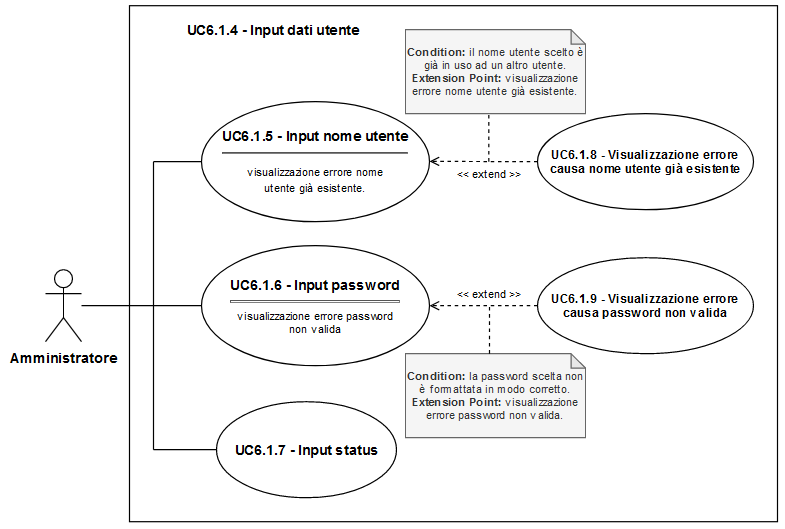
\includegraphics[width=15cm]{images/UC6.1.4.png}
		\caption{Diagramma UC6.1.4 - Input dati utente}
	\end{figure}
	\begin{itemize}
		\item \textbf{Attori primari:} utente amministratore;
		\item \textbf{Descrizione:} l'amministratore inserisce i dati dell'utente che ha intenzione di creare;
		\item \textbf{Scenario principale:} 
			\begin{itemize}
				\item l'amministratore esegue l'input del nome utente (UC6.1.5);
				\item l'amministratore esegue l'input della password (UC6.1.6).
			\end{itemize}
		\item \textbf{Precondizione:} l'amministratore sta compilando i dati del nuovo utente;
		\item \textbf{Postcondizione:} i dati dell'utente risultano inseriti nel sistema.
	\end{itemize}

\subsubsection{UC6.1.5 - Input nome utente}
	\begin{itemize}
		\item \textbf{Attori primari:} utente amministratore;
		\item \textbf{Descrizione:} l'amministratore inserisce il nome utente del nuovo utente che ha intenzione di creare;
		\item \textbf{Scenario principale:} l'amministratore esegue l'input del nome utente;
		\item \textbf{Precondizione:} l'amministratore sta compilando i dati del nuovo utente;
		\item \textbf{Postcondizione:} il nome dell'utente risulta inserito.
		\item \textbf{Estensione:}
		\begin{itemize}
			\item \textbf{UC6.1.8:} se si tenta di usare un nome utente già esistente, viene visualizzato un apposito messaggio di errore.
		\end{itemize}
	\end{itemize}

\subsubsection{UC6.1.6 - Input password}
	\begin{itemize}
		\item \textbf{Attori primari:} utente amministratore;
		\item \textbf{Descrizione:} l'amministratore inserisce la password del nuovo utente che ha intenzione di creare;
		\item \textbf{Scenario principale:} l'amministratore esegue l'input della password;
		\item \textbf{Precondizione:} l'amministratore sta compilando i dati del nuovo utente;
		\item \textbf{Postcondizione:} la password dell'utente risulta inserita.
		\item \textbf{Estensione:}
		\begin{itemize}
			\item \textbf{UC6.1.9:} se si tenta di creare una password che non rispetta le regole di formattazione stabilite, viene visualizzato un apposito messaggio di errore.
		\end{itemize}
	\end{itemize}

\subsubsection{UC6.1.7 - Input status}
\begin{itemize}
	\item \textbf{Attori primari:} utente amministratore;
	\item \textbf{Descrizione:} l'amministratore sceglie se assegnare all'utente interessato lo status di amministratore oppure di utente autenticato;
	\item \textbf{Scenario principale:} l'amministratore specifica, tra le opzioni disponibili, lo status da assegnare all'utente;
	\item \textbf{Precondizione:} l'amministratore sta compilando i dati del nuovo utente;
	\item \textbf{Postcondizione:} lo status dell'utente risulta inserito.
\end{itemize}

\subsubsection{UC6.1.8 - Visualizzazione errore causa nome utente già esistente}
	\begin{itemize}
		\item \textbf{Attori primari:} utente amministratore;
		\item \textbf{Descrizione:} l'amministratore visualizza un errore, relativo al fatto che il nome utente che ha tentato di assegnare all'utente è già in uso;
		\item \textbf{Scenario principale:} l'amministratore tenta di inserire un nome utente non valido in quanto assegnato ad un altro utente, ed il sistema risponde con un apposito errore;
		\item \textbf{Precondizione:} il nome utente scelto è già in uso ad un altro utente;
		\item \textbf{Postcondizione:} viene visualizzato un errore per informare l'utente che è necessario scegliere un altro nome utente.
	\end{itemize}

\subsubsection{UC6.1.9 - Visualizzazione errore causa password non valida}
	\begin{itemize}
		\item \textbf{Attori primari:} utente amministratore;
		\item \textbf{Descrizione:} l'amministratore visualizza un errore, relativo al fatto che la password che ha tentato di assegnare all'utente non è valida;
		\item \textbf{Scenario principale:} l'amministratore tenta di inserire una password non valida, ed il sistema risponde con un apposito errore;
		\item \textbf{Precondizione:} la password scelta non è formattata in modo corretto;
		\item \textbf{Postcondizione:} viene visualizzato un errore per informare l'utente che è necessario scegliere una nuova password.
	\end{itemize}

\subsubsection{UC6.2 - Gestione mappatura ambiente}
	\begin{itemize}
		\item \textbf{Attori primari:} utente amministratore;
		\item \textbf{Descrizione:} l'amministratore visiona la mappatura dell'ambiente, ed applica le modifiche volute tramite l'uso di un file appositamente formattato;
		\item \textbf{Scenario principale:} l'amministratore importa l'opportuno file per l'impostazione della mappatura dell'ambiente gestito dal sistema;
		\item \textbf{Precondizione:} l'amministratore visualizza lo stato attuale della mappa;
		\item \textbf{Postcondizione:} la mappa, rispetto allo stato iniziale, risulta modificata come voluto.
		\item \textbf{Estensione:}
		\begin{itemize}
			\item \textbf{UC6.2.1:} se si tenta di usare un file non valido per l'impostazione della mappa, viene visualizzato un apposito messaggio di errore.
		\end{itemize}
	\end{itemize}

\subsubsection{UC6.2.1 - Visualizzazione errore causa file non valido}
	\begin{itemize}
		\item \textbf{Attori primari:} utente amministratore;
		\item \textbf{Descrizione:} l'amministratore visualizza un errore, relativo al fatto che il file che si è cercato di usare per impostare la mappa non è stato formattato correttamente;
		\item \textbf{Scenario principale:} l'amministratore tenta di importare un file non valido per l'impostazione della mappa;
		\item \textbf{Precondizione:} l'amministratore tenta di modificare lo stato della mappa;
		\item \textbf{Postcondizione:} viene visualizzato un errore per informare l'utente che le modifiche alla mappa sono fallite a causa di errori nel file di importazione.
	\end{itemize}

\subsubsection{UC6.3 - Gestione lista unità}
	\begin{figure}[h!]
		\centering
		\includegraphics[width=16cm]{images/UC6.3.png}
		\caption{Diagramma UC6.3 - Gestione lista unità}
	\end{figure}
	\begin{itemize}
		\item \textbf{Attori primari:} utente amministratore;
		\item \textbf{Descrizione:} l'amministratore visiona la lista delle unità presenti nel sistema, ed applica le modifiche volute;
		\item \textbf{Scenario principale:} 
			\begin{itemize}
				\item l'amministratore inserisce un'unità (UC6.3.1);
				\item l'amministratore modifica un'unità (UC6.3.2);
				\item l'amministratore elimina un'unità (UC6.3.3).
			\end{itemize}
		\item \textbf{Precondizione:} l'amministratore visualizza l'elenco delle unità esistenti;
		\item \textbf{Postcondizione:} la lista delle unità risulta modificata come voluto rispetto allo stato iniziale.
	\end{itemize}

\subsubsection{UC6.3.1 - Inserimento unità}
	\begin{itemize}
		\item \textbf{Attori primari:} utente amministratore;
		\item \textbf{Descrizione:} l'amministratore intende aggiungere una nuova unità, alla lista di quelle gestite dal sistema;
		\item \textbf{Scenario principale:} l'amministratore aggiunge l'unità interessata alla lista di quelle già esistenti;
		\item \textbf{Precondizione:} l'amministratore visualizza l'elenco delle unità esistenti;
		\item \textbf{Postcondizione:} la lista delle unità risulta aggiornata con l'aggiunta dell'unità interessata.
		\item \textbf{Estensione:}
		\begin{itemize}
			\item \textbf{UC6.3.4:} se si tenta di usare l'ID di un'unità già esistente, viene visualizzato un apposito messaggio di errore.
		\end{itemize}
	\end{itemize}

\subsubsection{UC6.3.2 - Modifica unità}
	\begin{itemize}
		\item \textbf{Attori primari:} utente amministratore;
		\item \textbf{Descrizione:} l'amministratore intende modificare le proprietà di un'unità già esistente;
		\item \textbf{Scenario principale:} l'amministratore modifica le proprietà dell'unità interessata;
		\item \textbf{Precondizione:} l'amministratore visualizza l'elenco delle unità esistenti;
		\item \textbf{Postcondizione:} le proprietà dell'unità interessata risultano aggiornate come voluto.
		\item \textbf{Estensione:}
		\begin{itemize}
			\item \textbf{UC6.3.4:} se si tenta di usare l'ID di un'unità già esistente, viene visualizzato un apposito messaggio di errore.
		\end{itemize}
	\end{itemize}

\subsubsection{UC6.3.3 - Rimozione unità}
	\begin{itemize}
		\item \textbf{Attori primari:} utente amministratore;
		\item \textbf{Descrizione:} l'amministratore intende eliminare un'unità, dalla lista di quelle gestite dal sistema;
		\item \textbf{Scenario principale:} l'amministratore cancella l'unità interessata dalla lista di quelle esistenti;
		\item \textbf{Precondizione:} l'amministratore visualizza l'elenco delle unità esistenti;
		\item \textbf{Postcondizione:} la lista delle unità risulta aggiornata con la rimozione dell'unità interessata.
	\end{itemize}

\subsubsection{UC6.3.4 - Visualizzazione errore causa ID unità già esistente}
	\begin{itemize}
		\item \textbf{Attori primari:} utente amministratore;
		\item \textbf{Descrizione:} l'amministratore visualizza un errore, relativo al fatto che l'ID che si è cercato di usare è già assegnato ad un'unità esistente;
		\item \textbf{Scenario principale:} l'amministratore tenta di inserire un ID non valido in quanto assegnato ad un'altra unità, ed il sistema risponde con un apposito errore;
		\item \textbf{Precondizione:} l'ID scelto è già in uso ad un altra unità;
		\item \textbf{Postcondizione:} viene visualizzato un errore per informare l'utente che è necessario scegliere un altro ID per l'unità.
	\end{itemize}